\section{Introduction}
%Introduce veritesting, present our simple example and its performance improvement, segue into how veritesting at Java bytecode level is different from binary level
Symbolic execution is a popular testing technique that performs non-standard execution of a program.
%
Having been originally proposed in the 1970s, it has many applications
like test generation~\cite{dart,cute}, equivalence checking~\cite{ramos,adaptorsynth}, finding vulnerabilities~\cite{driller,angr}, checking correctness of transport protocols~\cite{transport}.
%
However, scalability continues to remain a challenge for symbolic execution.
%
Dynamic state merging~\cite{kuznetsov} provides one way to
alleviate scalability challenges by opportunistically merging dynamic
symbolic executors.
%
Veritesting~\cite{veritesting} is a different recently proposed
technique that is more suitable to symbolic execution tools that execute
one path at a time.
%
It has been shown to find more bugs, and achieve more node and path coverage, when implemented at the X86 binary level.
%
This provides motivation for investigating integration of veritesting with symbolic execution at the Java bytecode level.

\lstinputlisting[caption={An example to loop through a symbolic array with three execution paths through the loop body},
label={lst:v_ex}]{code_samples/VeritestingPerf.java}

Symbolic Pathfinder~(SPF)~\cite{spf} is a tool that performs symbolic execution of Java bytecode.
%
%SPF is tightly integrated with Java PathFinder~(JPF)~\cite{jpf} and uses JPF extensions to replace concrete execution with symbolic execution.
%
We present an example demonstrating the potential benefit of integrating veritesting with SPF in Listing~\ref{lst:v_ex}.
%
It checks if positive or negative integers occur more frequently in the
array~\textit{x}.
%
But, Listing~\ref{lst:v_ex} contains a bug if \textit{x} contains an
equal number of positive and negative integers.
%
The three-way branch on lines 5, 6 causes the total number of execution
paths required to cover the \textit{for} loop to be $3^{\textit{len}}$.
%
However, this three-way branch can be combined into a multi-path region
and represented as a predicate.
%
Each iteration through the loop can be represented by such a predicate.
%
We present such predicates in SMT2 notation in
Listing~\ref{lst:v_ex_smt2} assuming \textit{x} to contain two symbolic
integers named \textit{x0} and \textit{x1}~(\textit{len} equals 2).
%
The updates to \textit{sum} in the two loop iterations are captured by
\textit{sum0} and \textit{sum1}.
%
Using such predicates to represent the three-way branch on lines 5, 6 of
Listing~\ref{lst:v_ex} allows us to have only one execution path through
the loop body.
%
Figure~\ref{fig:v_ex_plot} shows a comparison of the number of execution
paths explored to find the bug on line 11 of Listing~\ref{lst:v_ex}.
%
The exponential speed-up from our predicates, representing multi-path
region, allows us to find
the bug using just three test cases.
%
Veritesting provides a way to get such performance improvements by using
static analysis to identify multi-path
regions and create predicates to represent them.
%
\lstinputlisting[caption={SMT2 representation of multi-path execution in
Listing ~\ref{lst:v_ex} using \textit{len} = 2}, label={lst:v_ex_smt2}, language=lisp]{code_samples/ex.smt2.snippet}
%
\begin{figure}[]
\caption{Comparing number of execution paths from Listing~\ref{lst:v_ex} using vanilla SPF and SPF with static unrolling}
\label{fig:v_ex_plot}
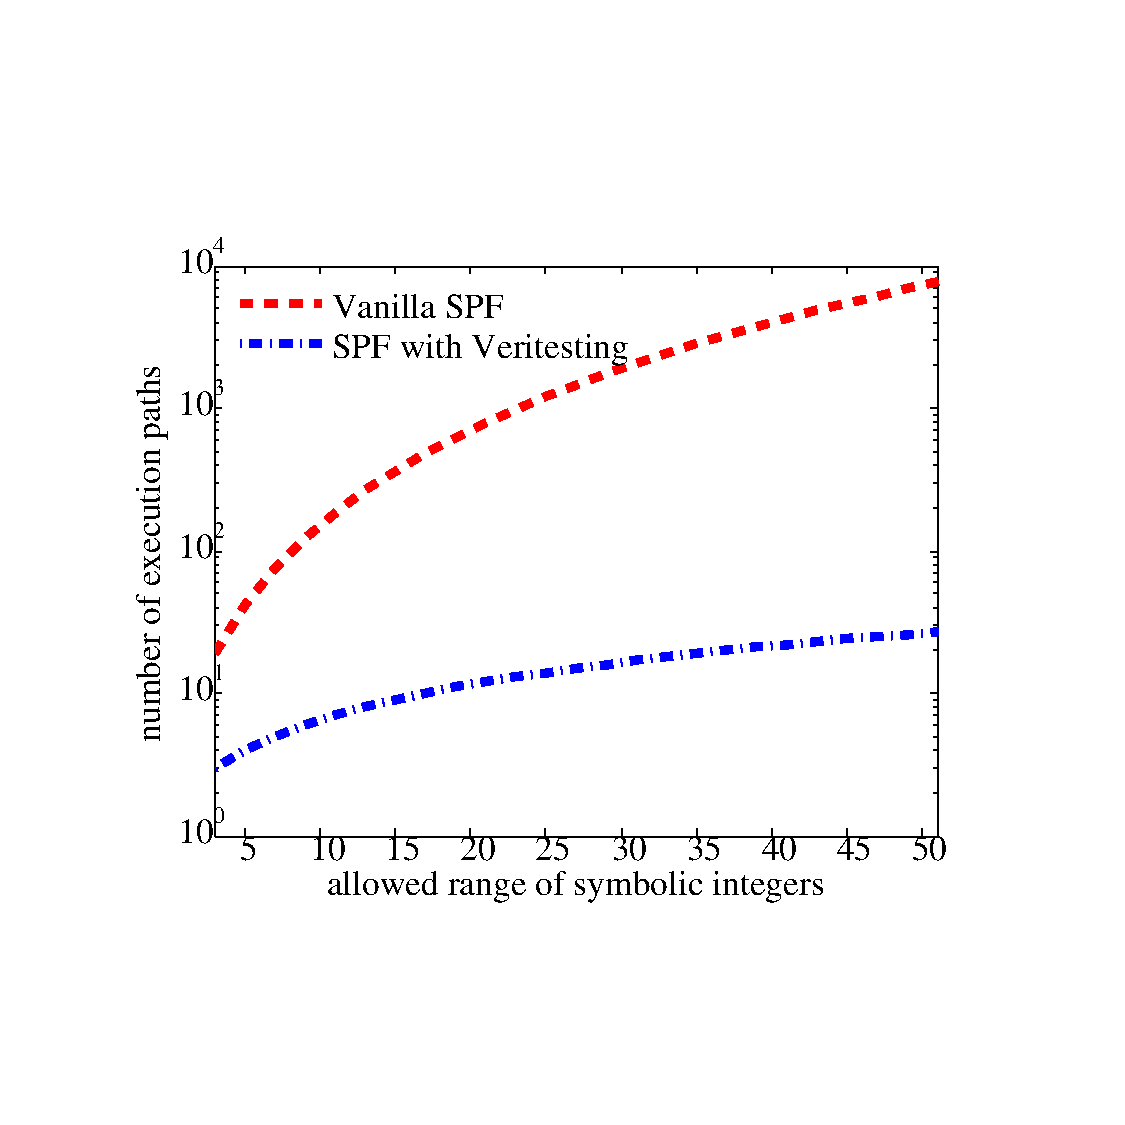
\includegraphics[width=\columnwidth]{figures/veritesting_example_semilogy}
\end{figure}
%
